\documentclass[11pt, a4paper]{article}
\usepackage[utf8]{inputenc}
\usepackage{amsmath,setspace,geometry}
\usepackage{amsthm}
\usepackage{amsfonts}
\usepackage{mathtools}
\mathtoolsset{showonlyrefs}
\usepackage[shortlabels]{enumitem}
\usepackage{rotating}
\usepackage{pdflscape}
\usepackage{graphicx}
\usepackage{bbm}
\usepackage[dvipsnames]{xcolor}
\usepackage[colorlinks=true, linkcolor= RawSienna, citecolor = RawSienna, filecolor = RawSienna, urlcolor = RawSienna, hypertexnames = true, backref = page]{hyperref}
\usepackage[]{natbib} 
\bibpunct[:]{(}{)}{,}{a}{}{,}
\geometry{left = 1.0in,right = 1.0in,top = 1.0in,bottom = 1.0in}
\usepackage[english]{babel}
\usepackage{float}
\usepackage{caption}
\usepackage{subcaption}
\usepackage{tikz}
\usepackage{booktabs}
\usepackage{pdfpages}
\usepackage{threeparttable}
\usepackage{lscape}
\usepackage{bm}
\setstretch{1.3}
%\usepackage[tablesfirst,nolists]{endfloat}

\usepackage[T1]{fontenc}
\usepackage{mlmodern}  % 太いComputer Modern
% MLmodernのバグを修正: cf. https://tex.stackexchange.com/questions/646333/size-of-integral-symbol-in-section-header-with-mlmodern
\DeclareFontFamily{OMX}{mlmex}{}
\DeclareFontShape{OMX}{mlmex}{m}{n}{<->mlmex10}{} 
\usepackage{tgtermes} % 数式以外の欧文をTXフォントで上書き

\newtheorem{theorem}{Theorem}
\newtheorem{assumption}{Assumption}
\newtheorem{lemma}{Lemma}
\newtheorem{definition}{Definition}
\newtheorem{proposition}{Proposition}
\newtheorem{claim}{Claim}
\newtheorem{corollary}{Corollary}
\newtheorem{example}{Example}
\DeclareMathOperator{\rank}{rank}

\theoremstyle{remark}
\newtheorem{remark}{Remark}


\title{Note on Conduct Parameter Estimation}
\author{Yuri Matsumura\thanks{Department of Economics, Rice University, \href{mailto:}{yuri.matsumura23@gmail.com}} \and Suguru Otani \thanks{Market Design Center, Department of Economics, University of Tokyo, \href{mailto:}{suguru.otani@e.u-tokyo.ac.jp}
\\Declarations of interest: none %this is for Economics Letters
}}

\begin{document}

\maketitle

\noindent\textbf{Keywords:} Conduct parameters, Homogenous Goods Market, Monte Carlo simulation
\vspace{0in}
\newline
\noindent\textbf{JEL Codes:} C5, C13, L1

\bigskip


\section{Introduction}

Measuring market power is a fundamental task in Industrial Organization. 
The conduct parameter approach provides a robust framework for evaluating market power, and a substantial body of empirical research has focused on identifying this parameter. 
\cite{bresnahan1982oligopoly} and \citet{lau1982identifying} provide fundamental results on identifying the conduct parameter.
First, \citet{bresnahan1982oligopoly} establishes key conditions for identifying the conduct parameter in a homogeneous product market, assuming a linear demand function and linear marginal costs. 
Second, \citet{lau1982identifying} extends this identification framework by relaxing the linearity assumptions.

In this note, we provide a counterexample to the identification result in \citet{lau1982identifying}. 
The paper argues that the separability of the demand function, a concept introduced by \citet{goldmanNote1964}, is critical for identification. 
Specifically, the conduct parameter and the marginal cost function can be identified when the demand function is non-separable or follows a particular separable form.
In contrast, we identify a separable demand function that does not conform to the particular form yet still allows identification. 


In fact, the counterexample breaks the proof for the necessity of separability of the inverse demand function in \citet{lau1982identifying}.
While \citet{bresnahan1982oligopoly} proposes the identification result using demand rotation, demand rotation is unnecessary to identify the conduct parameter.
In fact, \citet{berry2014identification} illustrate an example where the change in marginal cost can be used to identify true firm conduct.







\section{Model}
Consider a homogeneous product market.
The aggregate inverse demand and aggregate marginal cost function are given as
\begin{align}
    P = f(Q, X^{d}), \label{eq:demand}
    \\
    MC = g(Q, X^{s}),\label{eq:marginal_cost}
\end{align}
where $Q$ is the aggregate quantity, $X^{d}$ and $X^{s}$ are the vector of exogenous variables.
Assume that $X^{d}$ and $X^{s}$ are exclusive, that is, there is no common variable in $X^{d}$ and $X^{s}$.
Then, we obtain the supply equation:
\begin{align}
     P + \theta\frac{\partial P(Q)}{\partial Q}Q = MC,\label{eq:supply_equation}
\end{align}
where $\theta\in[0,1]$, which is the conduct parameter. The equation nests perfect competition ($\theta=0$) and perfect collusion ($\theta=1$) (See \cite{bresnahan1982oligopoly}). 



\section{Bresnahan (1982)}
\citet{bresnahan1982oligopoly} consider a model with linear demand and linear marginal cost.
He essentially considers the following model:
\begin{align}
    P & = \alpha_0 - \alpha_1 Q + \alpha_2 Y + \varepsilon_d,\label{eq:bresnahan_demand} \\
    MC & = \beta_0 + \beta_1 Q + \beta_2 W + \varepsilon_s. \label{eq:bresnahan_marginal_cost}
\end{align}
Assume that $\alpha_1>0$ and $\beta_1 >0$.
The total revenue is 
\begin{align}
    TR(Q) = PQ = \alpha_0Q - \alpha_1 Q^2 + \alpha_2 YQ + \varepsilon_d Q,
\end{align}
and hence, the marginal revenue becomes
\begin{align}
    MR = \alpha_0 - 2\alpha_1 Q + \alpha_2 Y + \varepsilon_d. \label{eq:bresnahan_marginal_revenue}
\end{align}
Note that the slope of the marginal revenue is twice as steep as the demand function under a linear demand model.
Based on the first-order condition \eqref{eq:supply_equation}, the supply relation can be computed as
\begin{align}
    P + \theta (-\alpha_1) Q & = \beta_0 + \beta_1 Q  + \beta_2 W + \varepsilon_s\\
   P & = \beta_0 + (\beta_1 + \theta\alpha_1) Q  + \beta_2 W + \varepsilon_s.\label{eq:bresnahan_supply}
\end{align}

The intersection of \eqref{eq:bresnahan_demand} and \eqref{eq:bresnahan_supply} derives the equilibrium price and the equilibrium quantity.
For example, let's consider perfect competition ($\theta = 0$) and monopoly ($\theta = 1$).
When $\theta = 0$, \eqref{eq:bresnahan_supply} implies that $MR = MC$, and the equilibrium quantity under perfect competition is
\begin{align}
    Q^C = \frac{\alpha_0 + \alpha_2 Y - \beta_0 - \beta_2 W+ \varepsilon_d - \varepsilon_s}{\alpha_1 + \beta_1}
\end{align}
In contrast, the monopoly implies that $P = MR$, and the equilibrium quantity under monopoly is
\begin{align}
    Q^m = \frac{\alpha_0 + \alpha_2 Y - \beta_0 - \beta_2 W+ \varepsilon_d - \varepsilon_s}{2\alpha_1 + \beta_1}.
\end{align}

Let $(\beta_0^c, \beta_1^c, \beta_2^c)$ be the parameters of the marginal cost rationalizing the perfect competition and $(\beta_0^m, \beta_1^m, \beta_2^m)$ be that rationalizing monopoly. 
For example, suppose that $\beta_1^c = \alpha_1 + \beta_1^m$, which implies that the marginal cost rationalizing monopoly is flatter than the perfect competition cost.
In this case, the equilibrium quantity is the same in both models ($Q^c = Q^m$) for any values of exogenous variables and the error terms. 
Hence, the researcher cannot distinguish two models from the data.
Using the supply relation, we can also demonstrate that the conduct parameter cannot be identified.
Let $\gamma = (\beta_1 + \theta \alpha_1)$.
Then, the parameters can be identified in \eqref{eq:bresnahan_supply} are $\beta_0$,$\gamma$, and $\beta_2$, but we cannot identify $\theta$ as $\gamma$ in both models has the same value of $\gamma$ because
\begin{align}
    \gamma^c = \beta_1^c + 0 \cdot \alpha_1 = \beta^c_1 = \beta_1^m + 1 \cdot \alpha_1 = \gamma^m.
\end{align}




Figure \ref{fig:bresnahan_non_identification} illustrates this situation.
Let $MC^c$ be the marginal cost rationalized by the perfect competition and $MC^m$ be the marginal cost rationalized by the monopoly.
$E_1$ is the observed equilibrium outcome, and both models rationalize the equilibrium.
Furthermore, the demand shift does not help identify the conduct, which equally increases the quantity under both perfect competition and monopoly, and $E_2$, the new equilibrium point, is still rationalized by both models.
Also, it is easy to see that the shift in the marginal cost function does not help identify the conduct parameter.

\begin{figure}[th!]
    \begin{center}
    \begin{subfigure}[t]{0.42\textwidth}
        \centering
        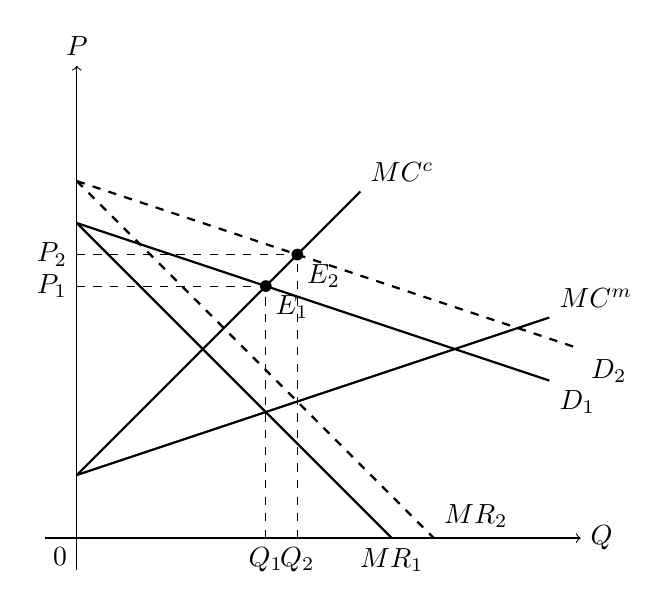
\begin{tikzpicture}[scale = 0.8]
        % Axes
        \draw[->] (-0.5,0) -- (8,0) node[right] {$Q$}; % Horizontal axis
        \draw[->] (0,-0.5) -- (0,7.5) node[above] {$P$}; % Vertical axis

        % Demand Curve (D_1) - passes through (0,5), (3,4), and (7.5,2.5)
        \draw[thick] (0,5) -- (7.5,2.5) node[below right] {$D_1$};

        % Marginal Revenue (MR_1) - passes through (0,5), (3,2), and (5,0)
        \draw[thick] (0,5) -- (5,0) node[below] {$MR_1$};

        % Supply Curve under competition (S^c) - passes through (0,1), (3,4), and (4.5,5.5)
        \draw[thick] (0,1) -- (4.5,5.5) node[above right] {$MC^c$};

        % Supply Curve under monopoly (S^m) - passes through (0,1), (3,2), and (7.5,3.5)
        \draw[thick] (0,1) -- (7.5,3.5) node[above right] {$MC^m$};

        % Equilibrium point (E_1) - intersection of D_1 and S^c at (3,4)
        \node[circle, fill, inner sep=1.5pt] (E1) at (3,4) {};
        \node[below right] at (E1) {$E_1$};

        \node[circle, fill, inner sep=1.5pt] (E2) at (3.5,4.5) {};
        \node[below right] at (E2) {$E_2$};

        % Shifted Demand Curve (D_1 shifted)
        \draw[thick, dashed] (0,34/6) -- (8,3) node[below right] {$D_2$};

        % Shifted MR (MR_1 shifted)
        \draw[thick, dashed] (0,34/6) -- (34/6,0) node[above right] {$MR_2$};

        % Dashed lines for price and quantity
        \draw[dashed] (3,0) -- (3,4);
        \draw[dashed] (0,4) -- (3,4);

        \draw[dashed] (3.5,0) -- (3.5,4.5);
        \draw[dashed] (0,4.5) -- (3.5,4.5);

        % Additional labels
        \node[below left] at (0,0) {0};
        \node[left] at (0,4) {$P_1$};
        \node[below] at (3,0) {$Q_1$};


        \node[left] at (0,4.5) {$P_2$};
        \node[below] at (3.5,0) {$Q_2$};
        \end{tikzpicture}
        \caption{The illustration of the non-identification result}
        \label{fig:bresnahan_non_identification}
    \end{subfigure}
    \hfill
    \begin{subfigure}[t]{0.45\textwidth}
        \centering
        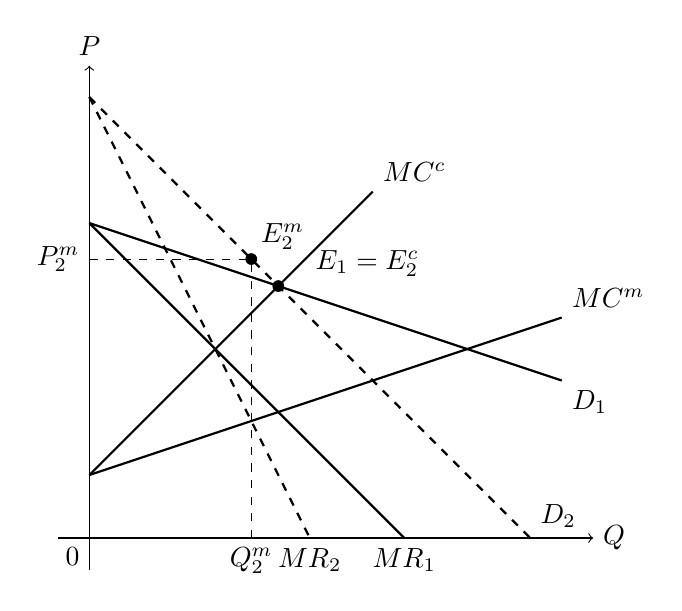
\begin{tikzpicture}[scale = 0.8]
        % Axes
        \draw[->] (-0.5,0) -- (8,0) node[right] {$Q$}; % Horizontal axis
        \draw[->] (0,-0.5) -- (0,7.5) node[above] {$P$}; % Vertical axis

        % Demand Curve (D_1) - passes through (0,5), (3,4), and (7.5,2.5)
        \draw[thick] (0,5) -- (7.5,2.5) node[below right] {$D_1$};

        % Marginal Revenue (MR_1) - passes through (0,5), (3,2), and (5,0)
        \draw[thick] (0,5) -- (5,0) node[below] {$MR_1$};

        % Supply Curve under competition (S^c) - passes through (0,1), (3,4), and (4.5,5.5)
        \draw[thick] (0,1) -- (4.5,5.5) node[above right] {$MC^c$};

        % Supply Curve under monopoly (S^m) - passes through (0,1), (3,2), and (7.5,3.5)
        \draw[thick] (0,1) -- (7.5,3.5) node[above right] {$MC^m$};

        % Equilibrium point (E_1) - intersection of D_1 and S^c at (3,4)
        \node[circle, fill, inner sep=1.5pt] (E1) at (3,4) {};
        \node[above right] at (E1) {$\quad E_1 = E_2^c$};

        % Equilibrium point (E_2) - intersection of D_1 and S^c at (7/2,9/2)
        \node[circle, fill, inner sep=1.5pt] (E2) at (18/7,7 - 18/7) {};
        \node[above right] at (E2) {$E_2^m$};
        \draw[dashed] (0,7 - 18/7) -- (18/7,7 - 18/7);
        \draw[dashed] (18/7,0) -- (18/7,7 - 18/7);

        % Shifted Demand Curve (D_1 shifted)
        \draw[thick, dashed] (0,7) -- (7,0) node[above right] {$D_2$};

        % Shifted MR (MR_1 shifted)
        \draw[thick, dashed] (0,7) -- (3.5,0) node[below] {$MR_2$};

        % Additional labels
        \node[below left] at (0,0) {0};
        \node[left] at (0,7 - 18/7) {$P_2^m$};
        \node[below] at (18/7,0) {$Q_2^m$};
        \end{tikzpicture}
        \caption{The illustration of the identification result}
        \label{fig:bresnahan_identification}
    \end{subfigure}
    \end{center}
    \caption{Comparison of the non-identification and identification results.}
    \label{fig:bresnahan_results}
    \vspace{2mm}
    \footnotesize
    Note: $MC^c$ is the marginal cost rationalized by the perfect competition, and $MC^m$ is the marginal cost rationalized by the perfect competition. 
    Assume that the true conduct is the perfect competition.
    The left figure illustrates the non-identification result. Perfect competition and monopoly generate the same equilibrium quantity and price at $E_1$, and even after a demand shift, both models generate the same equilibrium $E_2$.
    The right figure illustrates the identification result under the demand rotation instrument.
    The change in $Z$ changes the intercept and slope of the demand function without changing the equilibrium point under the true model.
    The shift due to the change in the demand rotation instrument leads to $D_2$ and $MR_2$.
    The new equilibrium under the perfect competition is still $E_1 = E_2^c$.
    The new equilibrium under the monopoly is now $E_2^m$, which is different from $E_2^c$.
\end{figure}




\subsection{Indentification}
To identify the conduct parameter, Bresnahan considers a shit of both the intercept and the slope of the demand function.
Consider the following demand function
\begin{align}
    P & = \alpha_0 - \alpha_1 Q + \alpha_2 Y - \alpha_3 QZ + \alpha_4 Z + \varepsilon_d,\\
    & = \alpha_0 - (\alpha_1 + \alpha_3Z) Q + \alpha_2 Y + \alpha_4 Z + \varepsilon_d. \label{eq:bresnahan_rotation_demand}
\end{align}
$Z$ shifts both the slope and the intercept of the inverse demand function and is called a demand rotation instrument.
The price elasticity includes $Z$ and is written as $-(\alpha_1 - \alpha_3 Z)$.
The supply relation is now
\begin{align}
    & P - \theta (\alpha_1 + \alpha_3Z) Q = \beta_0 + \beta_1 Q + \beta_2 W + \varepsilon_s\\
    \Longrightarrow &  P  = \beta_0 + (\beta_1 + \theta \alpha_1) Q  + \theta \alpha_3ZQ + \beta_2 W + \varepsilon_s.\label{eq:bresnahan_rotation_supply}
\end{align}
Let $\gamma = \beta_1 + \theta \alpha_1$ and $\kappa = -\theta \alpha_3$, and then the standard identification result implies that $\beta_0$, $\gamma$, $\kappa$, and $\beta_2$ in \eqref{eq:bresnahan_rotation_supply} are identified.
As $\alpha_1$ and $\alpha_3$ are both solely identified from the demand equation with appropriate demand instrument, $\theta$ and $\beta_1$ are also identified.


% 完全競争のときにZの変化がQを変化させないような数値の例を考えること.分母と分子の両方が変化するので,ちょっとめんどくさそう
% dQ/dzを計算してその微分係数がゼロになるような数値の設定であればよい


Figure \ref{fig:bresnahan_identification} illustrates the role of the demand rotation instrument.
The demand rotation instrument changes the slope and the intersection simultaneously.
Note that the marginal revenue is still twice as steep as the demand.
Assume that the true firm conduct is the perfect competition.
As the change in demand does not change the equilibrium point under perfect competition, the new equilibrium point under perfect competition $E_2^c$ is the same as the equilibrium point before the change $E_1$.
On the other hand, the equilibrium quantity under monopoly $Q_2^m$ is determined by the intersection of the marginal cost $MC^m$ and the new marginal revenue $MR_2$.
The equilibrium point under monopoly $E_2^m$ differs from $E_2^c$, so the conduct can be identified.


\subsection{Is demand rotation necessary for the identification of firm conduct?}

%結局,BresnahanとLauで考えているのはdemand sideの変化だけだけど,supply sideの変化でも同様にconduct parameterを識別する方法はある.
% Berry and HaileのSection 6の例では実際にmcの変化がconductの識別に利用できることを示している.
% Berry and HaileではMRを中心としたrotationでperfect copmetitionをrejectしているが,marginal revenueのrotationはdemandの傾きと切片も同時に変えることには注意
% Berry and Haileのtestable restrictionをconduct parameter identificationの条件とどう関連させるか?

% Berry and Haileでも"Following the literature, we consider the testability of specific models of firm conduct. This analysis can alternatively be interpreted as developing restrictions that can provide point identification or partial identification of the true model of conduct within a specified class of models. Open questions include what restrictions on the class of models would ensure point identification, and whether the restrictions we consider are exhaustive."
%と言っているので,Lauみたいにdemandに制限をかける,みたいなほうほうで点推定を達成するのはあり.


The idea in \citet{bresnahan1982oligopoly} is influential, but it is not a necessary condition.
For example, let's insert an instrument variable into the marginal cost function in the following way:
\begin{align}
    MC= \beta_0 + \beta_1 ZQ + \beta_2 W + \beta_3 Z + \varepsilon_s. \label{eq:marginal_cost_rotation}
\end{align}
In this marginal cost, the slope and the intercept are changed by the instrument variable, $Z$.
When the demand function is \eqref{eq:bresnahan_demand}, the supply equation under \eqref{eq:marginal_cost_rotation} becomes
\begin{align}
    & P - \theta\alpha_1 Q = \beta_0 + \beta_1 ZQ + \beta_2 W + \beta_3 Z + \varepsilon_s\\
    \Longrightarrow & P = \beta_0 + \beta_1 Z Q + \theta \alpha_1 Q + \beta_2 W + \beta_3 Z+ \varepsilon_s.
\end{align}
Obviously, the conduct parameter is identified under the supply equation.
Therefore, demand rotation is not a necessary condition but a sufficient one.






\section{Lau (1982)}
As the demand function can be identified, \citet{lau1982identifying} attempts to simultaneously identify both the conduct parameter and the marginal cost function through the supply equation \eqref{eq:supply_equation}. 
Instead of directly proving identification, \citet{lau1982identifying} takes an indirect approach by specifying the conditions under which the model is not identified. 
He defines non-identification in this model as follows:
\begin{definition}\label{def:non_identification}
    Non-identification implies
    \begin{align}
    f(Q, X^{d}) + \theta \frac{\partial f}{\partial Q}(Q, X^{d})Q &= g(Q, X^{s}),\label{eq:foc_alpha}\\
    f(Q, X^{d}) + \theta' \frac{\partial f}{\partial Q}(Q, X^{d})Q &= g'(Q, X^{s}), \label{eq:foc_beta}
    \end{align}
    where $\theta \neq \theta'$, $g \ne g'$,\footnote{This condition is not stated in \citet{lau1982identifying}, but assuming $g = g'$ makes the identification simple.} and the reduced form functions $Q = h(X^{d}, X^{s})$ and $Q = h'(X^{d}, X^{s})$ defined by \eqref{eq:foc_alpha} and \eqref{eq:foc_beta} respectively are identical.
\end{definition}
Intuitively, two models with different conduct parameters and marginal cost functions can generate the same equilibrium quantity and price. 
Therefore, the researcher cannot distinguish between the two models based solely on the observed data.

\citet{lau1982identifying} presents the condition on the demand function under which the conduct parameter cannot be identified:
\begin{theorem}\label{theorem_lau}
    Under the assumption that the industry inverse demand and cost functions are twice continuously differentiable, the index of competitiveness $\theta$ cannot be identified from data on industry price and output and other exogenous variables alone if and only if the industry inverse demand function is separable in $X^{d}$, that is,
    \begin{align}
        P = f(Q, r(X^{d})), \label{eq:demand_separable}
    \end{align}
    but not take the form, 
    \begin{align}
        P = Q^{-1/\theta}r(X^{d}) + s(Q). \label{eq:identification_separable}
    \end{align}
\end{theorem}
The theorem implies that the conduct parameter is identified when the demand function is not separable.
Even when the demand function is separable, the conduct parameter is identified if it satisfies \eqref{eq:identification_separable}.

\begin{remark}
    \citet{bresnahan1982oligopoly} considers a model with linear demand and marginal cost.
    He considers a demand function such that $P = \alpha_0 + (\alpha_1 + \alpha_2 Z) Q + \alpha_3 Y + \varepsilon$ where $Z$ is called a demand rotation instrument.
    It is easy to verify that this demand is not separable.
    Under the demand, the conduct parameter and the marginal cost parameter can be identified.
    \citet{matsumura2023resolving} provide more detailed conditions for the identification.
\end{remark}

\begin{remark}
    By Theorem 2 in \citet{goldmanNote1964}, \eqref{eq:demand_separable} implies that 
    \begin{align}
    \frac{\partial }{\partial Q} \left(\frac{\partial P/\partial X_{i}^{d}}{\partial P/\partial X_{j}^{d}} \right) = 0,\quad i \ne j, 
\end{align}
where $X_{i}^{d}$ is the $i$-th element in $X^{d}$.
\end{remark}

\section{A counterexample}

We show that the conduct parameter is identified when the inverse demand function is separable. 
Consider the following inverse demand function and marginal cost function:
\begin{align}
    P & = \exp(\varepsilon_{d}) Q^{\alpha_0} (X_{1}^{d})^{\alpha_1}(X_{2}^{d})^{\alpha_2}\label{eq:counter_demand}\\
    MC & = \exp(\varepsilon_{s})Q^{\beta_0} (X_{1}^{s})^{\beta_1} (X_{2}^{s})^{\beta_2},\label{eq:counter_mc}
\end{align}
where $\varepsilon_{d}$ and $\varepsilon_{s}$ satisfy the mean independence condition $E[\varepsilon_{d}|X^{d}, X^{s}] = E[\varepsilon_{s}|X^{d}, X^{s}] =0$. 
Assume that $\alpha_0 \ne -1/\theta$, so as not to satisfy the specific functional form \eqref{eq:identification_separable}.

The inverse demand \eqref{eq:counter_demand} is separable because
\begin{align}
    \frac{\partial }{\partial Q} \left(\frac{\partial P/\partial X_{1}^{d}}{\partial P/\partial X_{2}^{d}} \right) = \frac{\partial }{\partial Q} \left(\frac{\alpha_{1}\exp(\varepsilon_{d}) Q^{-\alpha_0} (X_{1}^{d})^{\alpha_1-1}(X_{2}^{d})^{\alpha_2}}{\alpha_2\exp(\varepsilon_{d}) Q^{-\alpha_0} (X_{1}^{d})^{\alpha_1}(X_{2}^{d})^{\alpha_2-1}} \right) =  \frac{\partial }{\partial Q}\left(\frac{\alpha_1}{\alpha_2} \frac{X_{2}^{d}}{X_{1}^{d}} \right)=0.
\end{align}
%According to Theorem \ref{theorem_lau}, the conduct parameter cannot be identified.

By taking the logarithm of the inverse demand \eqref{eq:counter_demand}, we have a log-linear demand equation such that 
\begin{align}
    \log P = \alpha_0 \log Q + \alpha_1 \log X_{1}^{d}  + \alpha_2 \log X_{2}^{d} + \varepsilon_{d}.\label{eq:counter_demand_equation}
\end{align}
The demand parameters can be identified when $X^s$ is a vector of exclusive demand instruments.
Thus, we can assume that $\alpha_0, \alpha_1$, and $\alpha_2$ are known.  

The left-hand side of the first-order condition \eqref{eq:supply_equation} can be written as
\begin{align}
    P + \theta\frac{\partial P(Q)}{\partial Q}Q & =  P + \theta [\alpha_0 \exp(\varepsilon_{d})Q^{\alpha_0-1}(X_{1}^{d})^{\alpha_1}(X_{2}^{d})^{\alpha_2}] Q\\
    & = P + \theta \alpha_0 P\\
    &= (1 + \theta\alpha_0) P.
\end{align}
Substituting this and the marginal cost function \eqref{eq:counter_mc} into the supply equation \eqref{eq:supply_equation} and taking a logarithm, we obtain the log-linear supply equation,
\begin{align}
    \log P = - \log(1 + \theta\alpha_0) + \beta_0 \log Q + \beta_1 \log X_{1}^{s}+\beta_2 \log X_{2}^{s} + \varepsilon_{s}.\label{eq:counter_supply_equation}
\end{align}
Let $\gamma = - \log(1 + \theta\alpha_0)$. When $X^d$ and $X^s$ contain non-overlapping variables, $X^d$ serves as a vector of instrumental variables for the supply equation. 
Applying the identification argument for instrumental variable regression, the parameters in Equation \eqref{eq:counter_supply_equation}, namely $\gamma$, $\beta_0$, and $\beta_1$, are identified. 
Consequently, the parameter $\theta$ is also identified as $\theta = (\exp(-\gamma) - 1)/\alpha_0$, which contradicts Theorem \ref{theorem_lau}. 
%Note that we do not need to introduce Bresnahan demand rotation instruments, discussed in \cite{matsumura2023resolving}.

A critical remark is that the demand function exhibits constant elasticity, and \citet{lau1982identifying} states in his conclusion that it is impossible to identify the conduct parameter under the demand function unless $\alpha_0 = -1/\theta$. 
When this happens in the counterexample, the constant term in \eqref{eq:counter_supply_equation} becomes $\gamma = -\infty$, so the supply equation can adequately defined.
Therefore, the counterexample achieves the identification under the condition where \citet{lau1982identifying} states it is impossible and cannot achieve the identification under the condition where he states it is possible.

\subsection{Interpretation}




Let's consider our case.
The simplified version of our example is the following:
\begin{align}
    P & = \exp(\varepsilon_{d}) Q^{-\alpha_0} Y^{\alpha_1},\label{eq:simple_demand} \\
    MC & = \exp(\varepsilon_{s}) Q^{\beta_0} W^{\beta_1}. \label{eq:simple_marginal_cost}
\end{align}
The total revenue is
\begin{align}
    TR = PQ = \exp(\varepsilon_{d}) Q^{-\alpha_0+1} Y^{\alpha_1},
\end{align}
and hence the marginal revenue is
\begin{align}
    MR = (-\alpha_0+1)\exp(\varepsilon_{d}) Q^{-\alpha_0} Y^{\alpha_1}
\end{align}
Take the logarithm of the demand and the marginal revenue, we have
\begin{align}
    \log P & = -\alpha_0 \log Q + \alpha_1 \log Y + \varepsilon_d,\\
    \log MR& = \log (1 -\alpha_0) -\alpha_0 \log Q + \alpha_1 \log Y + \varepsilon_d.
\end{align}
On the other hand, the supply relation becomes
\begin{align}
    \log P = -\log (1 - \theta \alpha_0) + \beta_0 \log Q + \beta_1 \log W + \varepsilon_s. \label{eq:simple_supply}
\end{align}

While the conduct parameter changes the slope of the supply relation in Bresnahan's example, the change in the conduct parameter shifts the supply relation in our example.
To make the model feasible, we assume that $1- \theta \alpha_0 >0$ for any $\theta \in [0,1]$.
Because $\alpha_0>0$ and $\theta \in [0,1]$, $1- \theta\alpha_0 <1$, which implies that $- \log(1- \theta\alpha_0) > 0$.
Then, for example, when we compare perfect competition and monopoly,  the supply relations under perfect competition and monopoly are parallel by $\log(1 - \alpha_0)$, and the supply relation under monopoly is shifted upward to the supply relation under perfect competition.

Note also that $\log (1 - \alpha_0)$ parallels the demand function and the marginal revenue, and the marginal revenue is shifted downwards.

Figure \ref{fig:simpe_identification} plots the above equations as in Bresnahan's example.
As we can see, under perfect competition and monopoly, the equilibrium quantities under the two models differ.






and the equilibrium quantity is given by
\begin{align}
    \log Q_t &= \frac{ \log (1 - \theta \alpha_0 ) + \alpha_1 \log Y_t - \beta_2 \log W_{t} + \varepsilon^{d} - \varepsilon^{c}}{\alpha_0 + \beta_0 }.\label{eq:quantity_loglinear}
\end{align}

\begin{figure}[t]
    \centering
        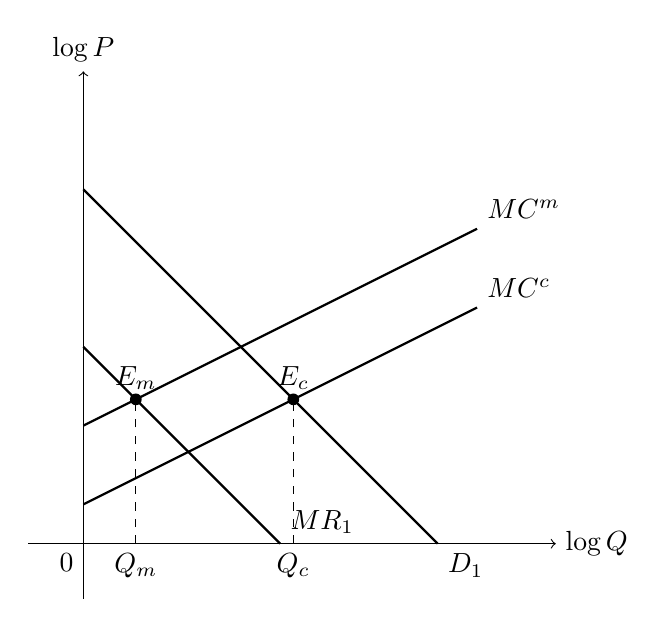
\begin{tikzpicture}
            % Axes
            \draw[->] (-0.7,0) -- (6,0) node[right] {$\log Q$}; % Horizontal axis
            \draw[->] (0,-0.7) -- (0,6) node[above] {$\log P$}; % Vertical axis

            % Marginal Revenue (MR_1) - passes through (0,5), (3,2), and (5,0)
            \draw[thick] (0,4.5) -- (4.5,0) node[below right] {$D_1$};
            \draw[thick] (0,2.5) -- (2.5,0) node[above right] {$MR_1$};
            
            % Supply Curve under competition (S^c) - passes through (0,1), (3,4), and (4.5,5.5)
            \draw[thick] (0,1.5) -- (5,4) node[above right] {$MC^m$};
            % Supply Curve under monopoly (S^m) - passes through (0,1), (3,2), and (7.5,3.5)
            \draw[thick] (0,0.5) -- (5,3) node[above right] {$MC^c$};

            % Equilibrium point (E_1) - intersection of D_1 and S^c at (3,4)
            \node[circle, fill, inner sep=1.5pt] (Ec) at (2/3,11/6) {};
            \node[above] at (Ec) {$E_m$};

            \node[circle, fill, inner sep=1.5pt] (Em) at (8/3,11/6) {};
            \node[above] at (Em) {$E_c$};
            % Additional labels
            \node[below left] at (0,0) {0};
            \node[below] at (2/3, 0) {$Q_m$};
            \node[below] at (8/3, 0) {$Q_c$};

            \draw[dashed] (8/3,0) -- (8/3,11/6);
            \draw[dashed] (2/3,0) -- (2/3,11/6);
        \end{tikzpicture}
        \caption{}
    \caption{Identification of the conduct under the log-linear model}
    \label{fig:simpe_identification}
\end{figure}



\bibliographystyle{aer}
\bibliography{conduct_parameter.bib}


\end{document}